\section{Introduction}
\AtBeginSection[]
{
	\begin{frame}<beamer>
		\frametitle{Plan}
		\tableofcontents[currentsection]
	\end{frame}
}

\begin{frame}{Introduction}
	\begin{block}{Lutra Consulting}
		\begin{itemize}
			\item Core QGIS developers
			\item General (GIS) software/web development
			\item Hydraulic modelling
		\end{itemize}
	\end{block}
\end{frame}

\section{QGIS}
\begin{frame}{About QGIS}
\begin{block}{What is it and what can it do?}
	\begin{itemize}
		\item Desktop, mobile and mapserver package:
		\begin{itemize}
			\item It's free
			\item It's Open Source
		\end{itemize}	
		\item QGIS can
		\begin{itemize}
			\item View GI
			\item Edit GI
			\item Present and publish GI
			\item Analyse GI
		\end{itemize}
		\item QGIS is
		\begin{itemize}
			\item Extensible (through plugins)
		\end{itemize}
		
	\end{itemize}
\end{block}
\end{frame}

\begin{frame}{Supported formats/services}
	\begin{block}{QGIS supports:}
		\begin{itemize}
			\item Vector files:
			\begin{itemize}
				\item ESRI Shapefile, Mapinfo MID/MIF or TAB, ESRI GDB, DXF,...
				\item PostGIS, MS SQL, Oracle Spatial, ...
			\end{itemize}	
			\item Raster files:
			\begin{itemize}
				\item TIF, PNG, ASCII, ECW, ESRI binary grid (HDR/ADF)
			\end{itemize}
			\item OGC services
			\begin{itemize}
				\item Web Mapping Service (WM(T)S)
				\item Web Feature Service (WFS)
				\item Web Processing Service (WPS, through plugin)
			\end{itemize}
		\end{itemize}
	\end{block}
\end{frame}

\begin{frame}{Editing/Digitizing}
	\begin{block}{More options than CAD software!}
		\begin{itemize}
			\item Numerical digitising
			\item Trace tool
			\item CAD tools
		\end{itemize}
	\end{block}
\end{frame}

\begin{frame}{Cartography}
	\begin{block}{Flexible styling}
		\begin{itemize}
			\item Rule-based labelling and styling
			\item Advanced Print Composer
			\item Catalogue/Atlas generator
		\end{itemize}
	\end{block}
\end{frame}

\begin{frame}{Processing}
	\begin{block}{Analysis and Geo-Processing}
		\begin{itemize}
			\item Over 600 modules
			\item Model builder
			\item Scripting
		\end{itemize}
	\end{block}
\end{frame}

\begin{frame}{Plugins}
	\begin{block}{Python plugins}
		\begin{itemize}
			\item 100s of existing plugins
			\item Easy to develop
		\end{itemize}
	\end{block}
\end{frame}

\begin{frame}{QGIS...}
	\begin{block}{So...why QGIS?}
		\begin{itemize}
			\item Why not?
		\end{itemize}
	\end{block}
\end{frame}

\section{Crayfish}
\subsection{What is Crayfish?}
\begin{frame}{About Crayfish}
	\begin{block}{ {
\includegraphics[width=0.2\textwidth]{crayfishlogo.png}}	}
		\begin{itemize}
			\item A C++/python QGIS plugin
			\item Reads temporal datasets
			\item Supports structured/unstructured mesh
		\end{itemize}
	\end{block}

\end{frame}

\subsection{Supported formats}
\begin{frame}{Supported file formats}
	\begin{block}{Hydraulic modelling packages:}
		\begin{itemize}
			\item SMS (Map) Output binary and ASCII (.dat Files)
				\begin{itemize}
					\item Hydro\_AS-2D
					\item BASEMENT
					\item TUFLOW
					\item Flood Modeller Pro 2D
				\end{itemize}
			\item Selafin files
					\begin{itemize}
						\item TELEMAC 2D
					\end{itemize}
			\item SWW format
					\begin{itemize}
						\item AnuGA
					\end{itemize}
			\item HDF format
					\begin{itemize}
						\item Hec RAS 2D
						\item TUFLOW (xmdf: based on HDF5)
					\end{itemize}
		\end{itemize}
	
	\end{block}
	
\end{frame}

\begin{frame}{Supported file formats}
	\begin{block}{Others(for used for metereology and oceanography):}
		\begin{itemize}
			\item NetCDF format
			\item Gridded Binary (GRIB)
		\end{itemize}
		
	\end{block}
\transduration<0-10>{0}
\multiinclude[<+->][format=png, graphics={width=\textwidth}]{grib}	


\end{frame}

\subsection{Features}

\subsubsection{Interface}
\begin{frame}{Contours}
	\begin{block}{Display gridded data}
		\begin{itemize}
			\item Various quantities
			\item Time slider
			\item Transparency
			\item Contour/vector/mesh options
			\item Mesh value tool
			
		\end{itemize}
		
	\end{block}
	
	\centering{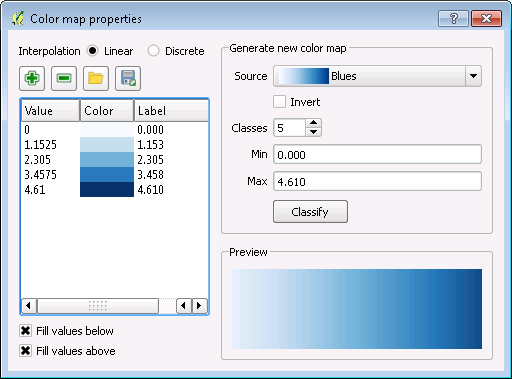
\includegraphics[width=0.5\textwidth]{crayfish_wiki_advanced_contour.png}}
	
\end{frame}

\subsubsection{Contours}

\begin{frame}{Contours}
	\begin{block}{Display gridded data}
		\begin{itemize}
			\item Styling and symbology
			\item Visible range
		\end{itemize}
		
	\end{block}

\centering{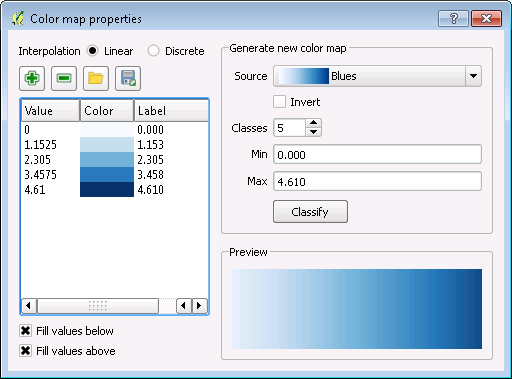
\includegraphics[width=0.5\textwidth]{crayfish_wiki_advanced_contour.png}}

\end{frame}